\FloatBarrier
\section{Reward Hacking in OPD: Convergence to a Biased Reward Signal}

\begin{figure}[t]
    \centering
    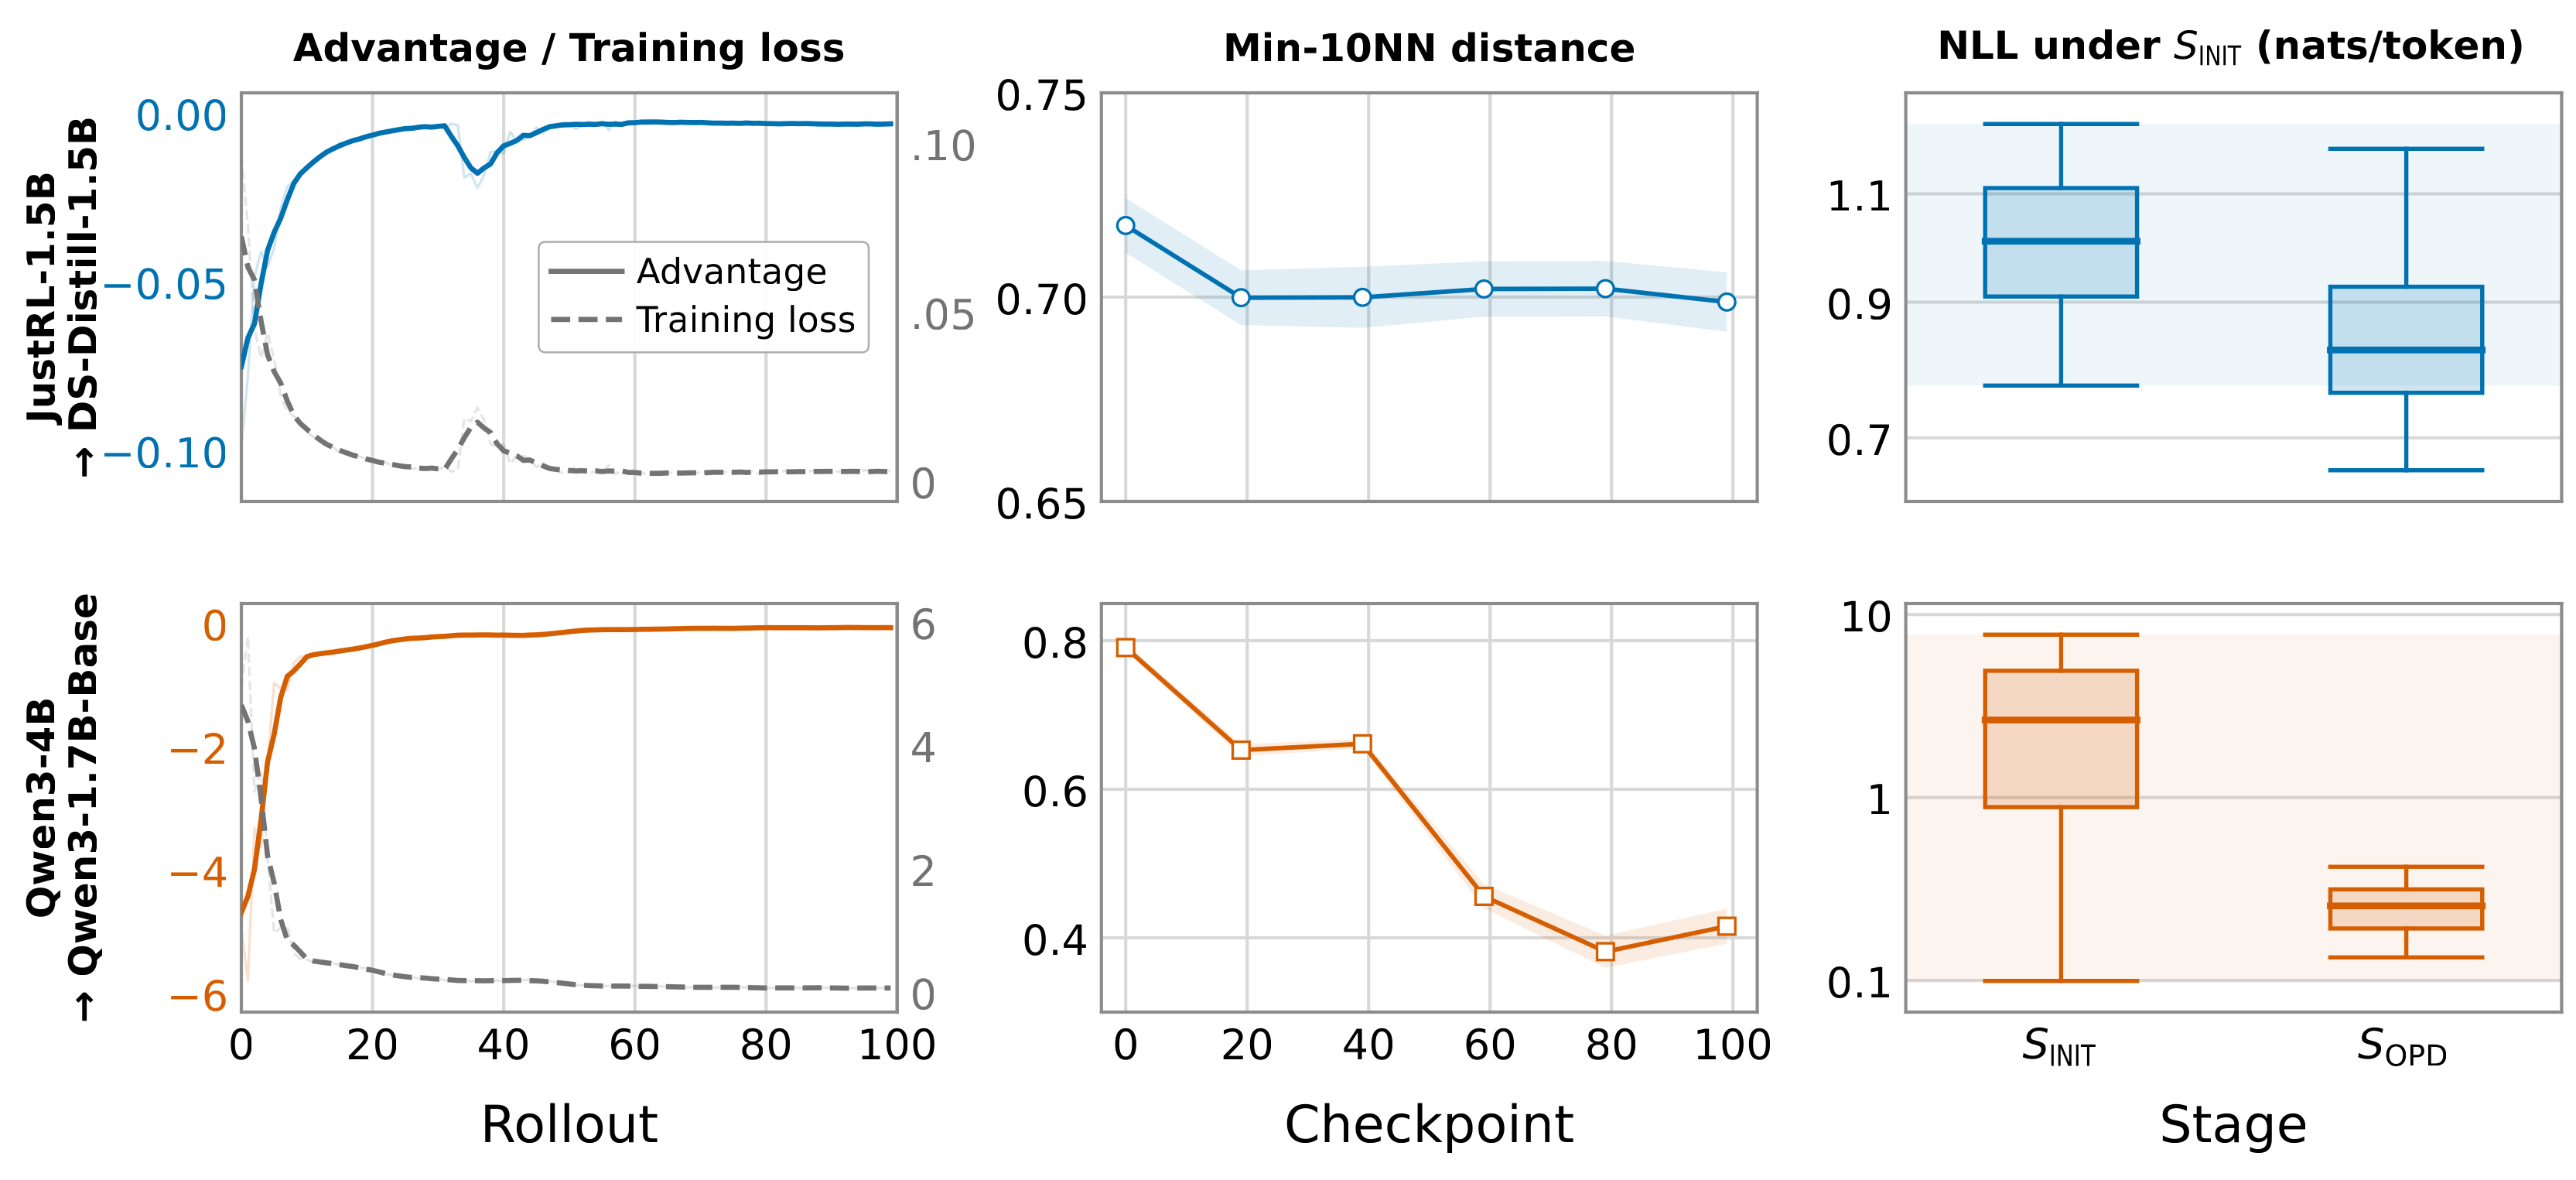
\includegraphics[width=0.95\textwidth]{S4/s4_convergence_overview_mpl.png}
    \caption{
        \textbf{Training process of the JustRL (top) and Qwen3-4B (bottom) settings.}
        Optimization converges normally in both settings, and the trained student's responses remain highly likely under $S_{\mathrm{INIT}}$.
        Columns: the advantage and training loss; the Min-10NN distance over six checkpoints; the NLL under $S_{\mathrm{INIT}}$ of responses from $S_{\mathrm{INIT}}$ and $S_{\mathrm{OPD}}$.
    }
    \label{figure_4_1}
\end{figure}

The preceding analysis shows that OPD improves performance without expanding the set of problems the student can solve.
Yet OPD training does not always succeed: some teacher-student pairs produce collapsed behaviors instead.
From a diagnostic perspective, we then examine whether the collapse constitutes reward hacking: optimization succeeding at the wrong target.
We first verify that the optimization converges normally, then characterize the behavioral shifts that emerge during training.

\subsection{Collapsed OPD Training Still Converges Normally}
\label{sec:4_1}

Our analysis starts by comparing a reported failure case of OPD with a successful one.
Prior work~\citep{li2026rethinkingopd} reports that OPD can fail when the teacher and student distributions are substantially mismatched, attributing the resulting degradation to this large distribution gap.
We therefore compare the full training process of the two settings:
the \textbf{JustRL setting} (JustRL-1.5B $\rightarrow$ DS-Distill-1.5B) where training improves the student,
and the \textbf{Qwen3-4B setting} (Qwen3-4B $\rightarrow$ Qwen3-1.7B-Base, without warm-up) where training collapses.
The loss and advantage in the Qwen3-4B setting converge as smoothly as those in the JustRL setting, with no qualitative difference in the shape of the curves.

We measure response concentration using the Min-10NN distance~\citep{zhang2026detectingrlvrtrainingdata}, which averages the ten smallest nearest-neighbor distances among responses to the same problem; lower values indicate greater similarity (described in detail in Appendix~\ref{app:response_geometry}).
The distance keeps decreasing during training in both settings: mildly in the JustRL setting, and much more sharply in the Qwen3-4B one.
Both students shrink toward a narrower space of behaviors, a phenomenon also reported in other work on on-policy RLVR post-training~\citep{yue2025does, zhao2025echochamberrlposttraining, dang2025assessing}.

If training exploits the reward rather than learning from it, the selected behaviors should already be accessible to $S_{\mathrm{INIT}}$ rather than genuinely novel.
To examine this, we compute the NLL under $S_{\mathrm{INIT}}$ for responses generated by the trained student and compare it with the NLL of $S_{\mathrm{INIT}}$'s own responses to the same problems.
Figure~\ref{figure_4_1} summarizes these diagnostics; the right panel reports this NLL comparison.
In both settings, the trained student's responses lie in the low NLL region of $S_{\mathrm{INIT}}$, which indicates that they are already familiar to $S_{\mathrm{INIT}}$.

\subsection{The Student Faithfully Fits the Reward Signal, Even When the Teacher Is Hacked}
\label{sec:4_2}

If the collapse constitutes reward hacking, the trained student should have successfully internalized the teacher's preferences, but those preferences should be misaligned with solution quality.

\begin{wraptable}{r}{0.48\textwidth}
    \centering
    \captionsetup{font=small}
    \begingroup
    \centering
    \scriptsize
    \setlength{\tabcolsep}{1.5pt}
    \vspace{-3mm}
    \renewcommand{\arraystretch}{1.08}

    \caption{
        \textbf{Endpoint generation characteristics on AIME24--26.}
        Model pairs denote teacher $\rightarrow$ student.
        Bold values mark length-limit saturation and severe repetition.
    }
    \label{tab:endpoint_generation_characteristics}

    \begin{tabular*}{\linewidth}{@{\extracolsep{\fill}}lrrrr@{}}
        \toprule
        Model & Acc. (\%) & Len. (k) & Trunc. (\%) & Rep. (\%) \\
        \midrule

        \rowcolor{black!6}
        \multicolumn{5}{@{}l}{\rule{0pt}{2.2ex}\textbf{JustRL-1.5B $\rightarrow$ DS-Distill-1.5B}} \\[1pt]
        Teacher & 39.3 & 9.30 & 13.8 & 0.0 \\

        $S_{\mathrm{INIT}}$ & 20.9 & 11.19 & 12.5 & 0.0 \\

        $S_{\mathrm{OPD}}$ & 37.1\,{\tiny(+16.2)} & 9.72 & 16.5 & 0.0 \\

        \midrule

        \rowcolor{black!6}
        \multicolumn{5}{@{}l}{\rule{0pt}{2.2ex}\textbf{Qwen3-4B $\rightarrow$ Qwen3-1.7B-Base}} \\[1pt]
        Teacher & 19.6 & 3.09 & 2.1 & 0.0 \\

        $S_{\mathrm{INIT}}$ & 0.2 & 1.18 & 4.1 & 4.2 \\

        $S_{\mathrm{OPD}}$ & 5.4\,{\tiny(+5.2)} & \textbf{8.16} & \textbf{99.4} & \textbf{38.0} \\

        \bottomrule
    \end{tabular*}
\endgroup

\end{wraptable}

\textbf{Endpoint behaviors are pathological.}
Table~\ref{tab:endpoint_generation_characteristics} compares the free generations of the teacher, $S_{\mathrm{INIT}}$, and $S_{\mathrm{OPD}}$ across both settings.
In the JustRL setting, the trained student's behaviors closely match the teacher's: accuracy improves by 16.2 points, and no severe repetition is detected.
In contrast, the Qwen3-4B setting exhibits a dramatically different outcome.
Although accuracy improves modestly (+5.2 points), nearly all responses hit the 8k generation limit (99.4\%), and 38\% exhibit severe repetition---far worse than either the teacher (2.1\% truncation, 0\% repetition) or $S_{\mathrm{INIT}}$ itself.
The trained student has not learned to reason like the teacher; instead, it has concentrated probability mass on a narrow subset of pathological behaviors.

\clearpage

\begin{wrapfigure}{r}{0.48\textwidth}
    \centering
    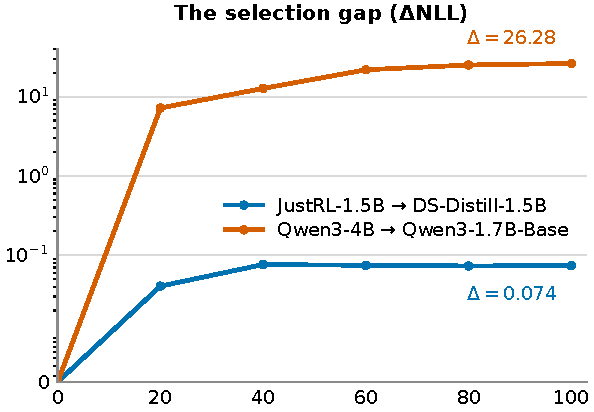
\includegraphics[width=0.9\linewidth]{S4/s4_2_selection_gap_no_ci.pdf}
    \captionsetup{font=small}
    \caption{
        \textbf{Selection gap before and after training.}
        Both students learn to discriminate teacher-preferred responses, with the Qwen3-4B setting showing overfitting.
    }
    \label{fig:selection_gap_comparison}
    \vspace{-5mm}
\end{wrapfigure}

\textbf{The trained student discriminates teacher-preferred responses.}
We measure how the trained student scores a fixed set of $S_{\mathrm{INIT}}$ responses.
We compare the 10\% of responses the teacher prefers most with the 10\% it prefers least, as ranked by teacher advantage.
For each response, $\Delta\text{NLL} = \text{NLL}_{S_t} - \text{NLL}_{S_0}$ measures the change in the student's NLL during training.
The \textit{selection gap} $\Gamma$ is the mean $\Delta\text{NLL}$ of the least-preferred 10\% minus that of the most-preferred 10\%.
A positive $\Gamma$ indicates that training favors the teacher's most-preferred responses over its least-preferred ones.

Figure~\ref{fig:selection_gap_comparison} shows whether this degradation reflects learned teacher preference rather than random drift. Both students increase their discrimination of teacher-preferred responses: JustRL's gap grows modestly from near zero to 0.07, while the Qwen3-4B setting's gap increases dramatically to approximately 26.
Combined with the endpoint generation table, this reveals that the student in the Qwen3-4B setting has \textit{overfit} to the subset of $S_{\mathrm{INIT}}$ responses that receive high teacher advantage but exhibit pathological behaviors.
